\section{Entity Relationship Diagram}

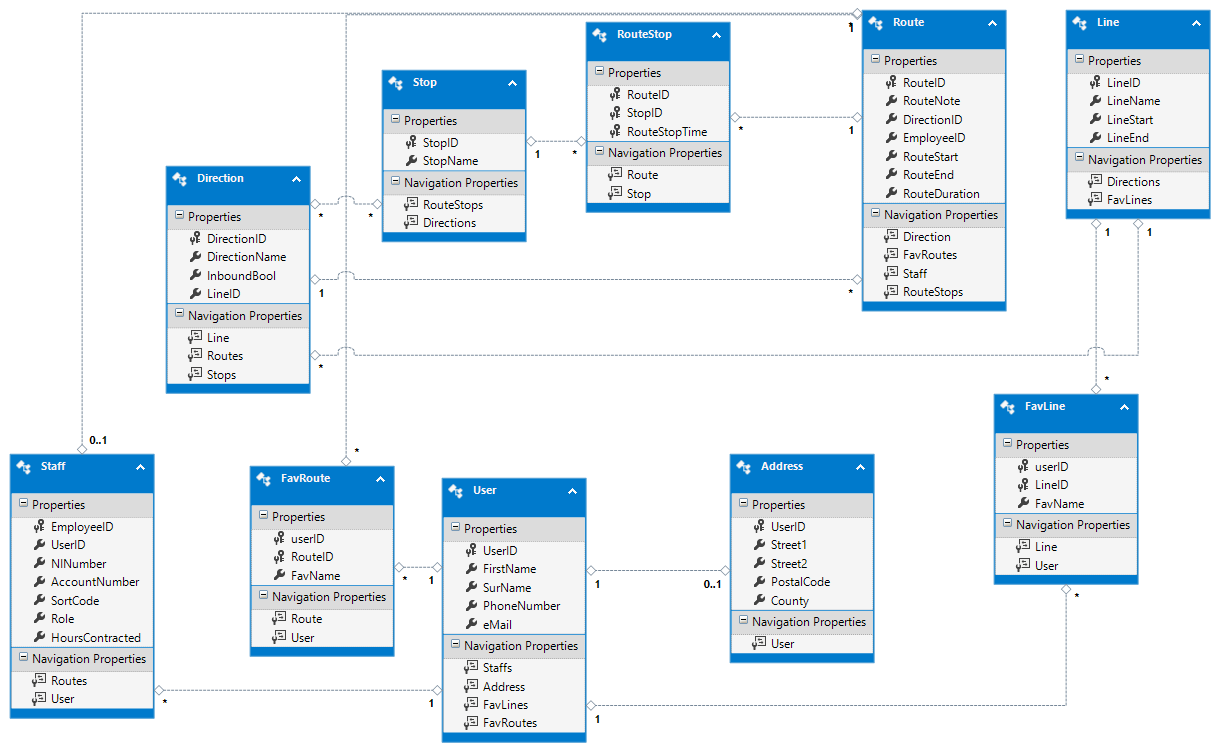
\includegraphics[width=\linewidth]{EntityDesignerDiagram.png}

\medskip

The Entity Relationship Diagram shows our revised database model
after multiple revisions.

\medskip

The $User$ entity has a $1$ to $0..1$ relation with the $Address$
table, where the address information was filled in during
registration (or later in account preferences) or not.

\medskip

Each $User$ entity has a one to many relationship with
$FavouriteRoute$ and $FavouriteLine$, which are association entities
to $Route$ and $Line$ respectively. These link multiple routes or
lines to a single user.

\medskip

A $Staff$ entity has a many to one relationship with the $User$
entity, as the $Staff$ entity extends the basic information stored
by the $User$ entity. However a $User$ may not have a relation with
the $Staff$ entity if they are just a customer.

\medskip

$Lines$ are the main entity for the bus timetabling system, where
a single line will have multiple $Directions$ (i.e. $A$ to $B$ and
$B$ to $A$).

\medskip

Each $Direction$ has many $Routes$, as each time slot a line
operates for is stored as its own route. For example, on $Line A$,
busses leaving at $0900$ and $0930$ are two separate routes assigned
to the same $Direction$ and $Line$ with different drivers.

\medskip

A $Direction$ also has many $Stops$, which contain the stop's name
and coordinates. However these stops may not be serviced by all of
the busses on the same line (e.g. limited services on weekends or
holidays). For this, there is another association entity called
$RouteStop$ which maps stops serviced by the $Line$ and stops the
$Route$ will actually be stopping at.
